%%Nagłówek pliku, konfiguracja stron

\documentclass[12pt,a4paper,oneside]{report} %default 10pt
\usepackage[utf8]{inputenc}
\usepackage{geometry} % to change the page dimensions
\usepackage{booktabs} % for much better looking tables
\usepackage{verbatim} % adds environment for commenting out blocks of text & for better verbatim
\usepackage{float}
\usepackage{amsfonts}
\usepackage{ifpdf}
\usepackage{indentfirst}
\usepackage{fancyhdr} % This should be set AFTER setting up the page geometry
\usepackage[T1]{fontenc}
\usepackage[utf8]{inputenc}

\def\dywiz{\kern0sp\discretionary{-}{-}{-}\penalty10000\hskip0sp\relax}
\def\prefacename{Przedmowa}
\def\refname{Bibliografia}
\def\abstractname{Streszczenie}
\def\bibname{Spis literatury}
\def\chaptername{Rozdział} % uppercasing in running head must work
\def\appendixname{Dodatek}
\def\contentsname{Spis tre\'sci}
\def\listfigurename{Spis rysunk\'ow}
\def\listtablename{Spis tabel}
\def\indexname{Skorowidz}
\def\figurename{Rysunek}
\def\tablename{Tabela}
\def\partname{Czę\'s\'c}
\def\enclname{Załaczniki}
\def\ccname{Do wiadomo\'sci}
\def\headtoname{Do}
\def\pagename{Strona}
\def\seename{Por\'ownaj}
\def\alsoname{Por\'ownaj tak\.ze}
\def\PLdateending{\space roku}
\def\today{\number\day~\ifcase\month\or
           stycznia\or lutego\or marca\or kwietnia\or maja\or czerwca\or
           lipca\or sierpnia\or wrze\'snia\or pa\'zdziernika\or
           listopada\or grudnia\fi \space\number\year \PLdateending}

\usepackage{caption}
\usepackage{mathtools}








\geometry{a4paper}
\geometry{margin=1in}
\pagestyle{plain}
\renewcommand{\headrulewidth}{0pt}
\lhead{}\chead{}\rhead{}
\lfoot{}\cfoot{\thepage}\rfoot{}
\setlength\parindent{24pt}

\usepackage{listings}
\lstset{literate={ć}{{\'c}}1 {ó}{{\'o}}1 {ś}{{\'s}}1 {ź}{{\'z}}1 {ń}{{\'n}}1
        {Ć}{{\'C}}1 {Ó}{{\'O}}1 {Ś}{{\'S}}1 {Ź}{{\'Z}}1 {Ń}{{\'N}}1
        {ą}{{\k{a}}}1 {ę}{{\k{e}}}1 {Ą}{{\k{A}}}1 {Ę}{{\k{E}}}1 {ż}{{\.z}}1
        {Ż}{{\.Z}}1 {ł}{{\l{}}}1 {Ł}{{\L{}}}1}

\usepackage{color}

\definecolor{dkgreen}{rgb}{0,0.6,0}
\definecolor{gray}{rgb}{0.5,0.5,0.5}
\definecolor{mauve}{rgb}{0.58,0,0.82}

\lstset{frame=tb,
    language=Python,
    aboveskip=3mm,
    belowskip=3mm,
    showstringspaces=false,
    columns=flexible,
    basicstyle={\small\ttfamily},
    numbers=none,
    numberstyle=\tiny\color{gray},
    keywordstyle=\color{blue},
    commentstyle=\color{dkgreen},
    stringstyle=\color{mauve},
    breaklines=true,
    breakatwhitespace=true,
    tabsize=3
}

\renewcommand\thechapter{\arabic{chapter}.}
\renewcommand\thesection{\arabic{chapter}\arabic{section}.}
\renewcommand\thesubsection{\arabic{chapter}\arabic{section}.\arabic{subsection}.}






















%%%%%%%%%%%%%%%%%%%%%%%%%%%%%%%%%%%%%%%%%%%%%%%%%%%%%%%%%%%%%%%%%%%%%%%%%%%
%%Praca właściwa

\begin{document}

\begin{titlepage}

\centering
\begin{tabular}{c}

\includegraphics[width=0.15\textwidth]{pg-logo.png}
\end{tabular}
\begin{tabular}{c}
Politechnika Gdańska \\
Wydział Fizyki i Matematyki Stosowanej
\end{tabular}
\par\vspace{1cm}

\begin{tabular}{c}
{\large Katedra Fizyki Teoretycznej i  Informatyki Kwantowej}\\
Fizyka Techniczna\\
Konwersja Energii\\
Studia Stacjonarne\\
\end{tabular}
\par\vspace{1cm}


{\scshape\LARGE Paweł Tomasik \par}
Nr albumu: 150243\par
\par\vspace{1cm}


\begin{tabular}{c}
{\small Projekt dyplomowy} \\

{\small inżynierski} \\
\end{tabular}
\par\vspace{1cm}


{\Large\scshape System doradztwa zawodowego z wykorzystaniem metod sztucznej inteligencji\par}
\vfill
Potwierdzenie przyjęcia projektu: \par
\vspace{1cm}
\begin{tabular}{ll}
Opiekun projektu & \hspace{5cm}  \\
dr Leszek Kułak &  \\
\end{tabular}
\par
\vspace{1cm}
\today

\end{titlepage}


{\centering\scshape Oświadczenie\par}
\vspace{1cm}
{
\raggedright
\begin{tabular}{ll}
Imię i nazwisko: & Paweł Tomasik \\
Wydział i kierunek: & FTiMS, Fizyka Techniczna \\
Data i miejsce urodzenia: & 10 stycznia 1994r., Kwidzyn \\
Adres: & Sokola 9/46, 82-500 Kwidzyn \\
Rodzaj studiów: & studia stacjonarne \\
\end{tabular}\hfill\par
}
\vspace{1cm}
Świadomy odpowiedzialności karnej z tytułu naruszenia ustawy z dnia 4 lutego 1994 r. o prawie autorskim i prawach pokrewnych
(Dz. U. Nr 80, poz. 904 z 2000r. ze zmianami) i konsekwencji dyscyplinarnych określonych w ustawie o szkolnictwie wyższym (Dz. U. Nr 164, poz. 1365 z 2005 r.), a także odpowiedzialności prawno-cywilnej, oświadczam, że przedkładana praca dyplomowa:\par 
\vspace{0.5cm}
{
    \scshape\noindent\itshape System doradztwa zawodowego z wykorzystaniem metod sztucznej inteligencji\par}
\vspace{0.5cm}
\noindent została opracowana przeze mnie samodzielnie i nie była podstawą żadnej innej urzędowej procedury związanej z nadaniem dyplomu wyższej uczelni lub tytułów zawodowych.\par
Oświadczam również, że niniejsza wersja pracy jest identyczna z załączoną wersją elektroniczną.\par
Wszystkie informacje umieszczone w pracy, uzyskane ze źródeł pisanych i elektronicznych, a także wszelkie inne informacje, zostały udokumentowane w wykazie literatury odpowiednimi odnośnikami, zgodnie z art. 34 ustawy o prawie autorskim i prawach pokrewnych. \par
Jednocześnie wyrażam zgodę na dołączenie tekstu pracy do bazy prac systemu antyplagiatowego. \par
Ponadto, wyrażam zgodę na wykorzystanie pracy dyplomowej do celów dydaktycznych i naukowych. \par
\vfill
{\centering
\begin{tabular}{lll}
Gdańsk, \today & \hspace{4cm} & Podpis autora \\
\end{tabular}
}
\vspace{1cm}
\pagebreak


















\renewcommand{\abstractname}{Strzeszczenie}
\begin{abstract}
Praca przedstawia system do przeprowadzania testów doradztwa zawodowego z wykorzystaniem metod analizy danych. Celem przyświecającym temu programowi jest zintegrowanie testów osobowości z technikami analizy danych i uczenia maszynowego. Napisana została aplikacja serwerowa, która umożliwia klientom wzięcie udziału w udostępnionym teście. Wyniki są zapisywane w logu i mogą być wykorzystywane do dalszej analizy. Możliwości narzędzi analitycznych oceniono na podstawie gotowego zestawu danych.
\par\vspace{2cm}
{\scshape Słowa kluczowe:} Uczenie maszynowe, klasyfikacja, data mining, model Hollanda \par
\end{abstract}

\renewcommand{\abstractname}{Abstract}
\begin{abstract}
This paper presents a vocational advisory system using data analytics. The goal of this system is to integrate personality tests with analytics and machine learning techniques. Server application was written, which enables users to take a test, of which results are logged for further analysis. Capabilities of used models were assessed basing on prepared dataset.
\par\vspace{2cm}
{\scshape Keywords:} Machine learing, classification, data mining, Holland model \par
\end{abstract}


\tableofcontents











\chapter{Testy osobowości jako problem analizy danych}

Kwestionariusze są jedną z najbardziej rozpowszechnionych metod badań społecznych, używaną także w formach nienaukowych w postaci tzw. psychotestów. Przykładami są np. \emph{Big Five} \cite{bigfive}, \emph{test Myers-Briggs} \cite{myersbriggs}, zaś z metod mniej formalnych - Enneagram \cite{enneagram}. \par

Kwestionariusze swoją popularność zawdzięczają przede wszystkim prostocie ich analizy - dane mają najczęściej charakter liczbowy, zazwyczaj wynikiem badania jest kategoria o największej sumie wyników. Badania te jako takie podlegają mniej lub bardziej, w zależności od użytych skal, narzędziom statystyki. \par

Na znamienną rolę analityki w badaniach społecznych(nie tylko psychologicznych) wskazuje istnienie takich platform jak \emph{Survey Monkey} \cite{surveymonkey}, które automatyzują podstawowe testy statystyczne i umożliwiają integrację z zewnętrznymi narzędziami statystycznymi. Natomiast prace takie jak \cite{test-postaw-milosnych} pokazują, że metody sztucznej inteligencji pozwalają udoskonalać metody psychometryczne.\par

W ostatnich czasach rola analizy danych znacząco wzrasta. Wraz z rozwojem komputeryzacji, objawiającym się rozwojem trendu IoT, wydajnymi metodami sztucznej inteligencji o szerokich zastosowaniach (więcej w dalszych częściach), metody statystyczne będące podstawą wnioskowania na danych stają się podstawą zaawansowanych systemów. Data mining jest nieodłączną częścią procesów przemysłowych związanymi z systemami \emph{Business Intelligence} i \emph{Big Data}. \par

Celem pracy jest zbudowanie systemu do iteracyjnej budowy i udoskonalania kwestionariuszy i testów osobowości na podstawie odpowiedzi do testu opartego o model RIASEC. W szczególności została wykonana analiza tych danych w celu przygotowania ich do modelowania, zbudowanie systemu do przeprowadzania testów wraz z uzyciem metod klasyfikacji i klasteryzacji oraz udostępnianiem danych do analizy oraz weryfikacja skuteczności użytych klasyfikatorów we wzajemnym porównaniu i w porównaniu do metryki testu.\par










\chapter{Zarys analizy danych}

Analiza danych jest dziedziną zajmującą się procesem wyciągania użytecznej informacji z danych poprzez ich transformację i modelowanie. Natomiast \emph{data mining} jest pojęciem z pogranicza uczenia maszynowego i statystyki. Jest ono różnie definiowanie przez autorów, zjednując je mniej lub bardziej z analizą danych. Niezależnie od definicji, celem obu tych dyscyplin jest odkrywanie wiedzy z danych, przechodzenie od szczegółu do ogółu. Przedstawione definicje wskazują na indukcyjny charakter wnioskowań wypływający z analiz - powstające modele generalizują dane.\par

Proces analizy składa się z kilku etapów, często nachodzących na siebie i powtarzających się. Poprawna analiza danych musi składać się ze zrozumienia analizowanej próbki, wstępnego przygotowania jej, modelowania i walidacji modelu. \par

\emph{CRISP-DM} stanowi przemysłowy standard wykorzystywania danych. Jego iteracyjna formuła jest dobrym punktem wyjścia do omówienia procesów związanych z danymi: ich zbieranie, zrozumienie, oczyszczanie, modelowanie i walidację. Iteracyjnośc procesu wynika z faktu, że opracowywane modele nie są doskonałe i podlegają ulepszaniu wraz z lepszym zrozumieniem badanych zjawisk. Jest to też powód, dla którego budowana platforma udostępnia raportowanie wyników. \cite{crispdm} \par

\begin{figure}
\centering
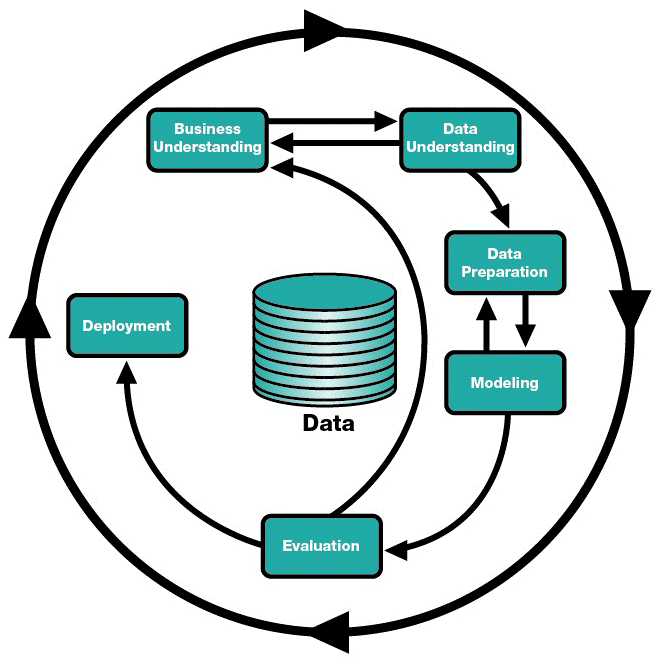
\includegraphics[width=0.5\textwidth]{crisp-dm.png}
\label{crisp-dm}
\caption{Metodologia CRISP-DM. Według \cite{crispdm} jedna z najpopularniejszych metodologii Data Miningu, implikuje wykorzystanie wiedzy do modelowania danych i poszerzanie wiedzy przez wnioski wyciągnięte z wykorzystania modelu. Modelowanie danych jest procesem iteracyjnym i dopiero po osiągnięciu odpowiedniej dokładności model jest wykorzystywany w produkcji.}
\end{figure}





\section{Techniki eksploracyjnej analizy danych}

Eksploracyjna analiza danych (EDA) stanowi etap przygotowawczy do budowy modelu na danych. Celem EDA jest sformułowanie i wstępne zweryfikowanie przez analityka założeń dotyczących danego problemu na podstawie trendów pojawiających się w próbce. EDA jest wykonywana jako etap poprzedzający \emph{confirmatory data analysis}. EDA jest też szeroko stosowana jako podstawa do budowania systemów Business Intelligence.\cite{hseltman} \par 

Wykorzystanie technik EDA zależy od rodzaju dostępnych danych oraz od oczekiwanego rodzaju wniosków. Przede wszystkim należy wyróżnić podział na metody \emph{numeryczne} i \emph{wizualne}. Te pierwsze stanowią nieparametryczne metody statystyczne. W szczególności jednak używane są techniki graficzne, pozwalające w łatwy sposób zobrazować kluczowe cechu zestawu danych: trendy, rozrzuty, odstępstwa, rozkłady etc. Techniki różnią się też w zależności od rodzaju danych i wymiarowości, w której operują.\par

Przed przejściem do omówienia poszczególnych technik należy zwrócić uwagę na rodzaje danych. Zgodnie ze \cite{stanisz-1}, wyróznia się cztery \emph{skale} danych: nominalną, porządkową, równomierną(interwałową) i ilorazową. Dane nominalne podlegają jedynie operacji równości i ich analiza jest najbardziej uproszczona. Dla danych porządkowych definiowalne są także relacje nierówności. Dane równomierne i ilorazowe pozwalają na dokładnie określenie odległości między punktami, przy czym dla skali ilorazowej da się określić punkt zerowy.\par

\subsection{Metody numeryczne}

Podstawą do analizy danych jest zestawienie próbki w postaci szeregu. W przypadku uszeregowania danych względem jakiejś zmiennej mówi się o szeregu szczegółowym. W opisanym zastosowaniu o wiele bardziej interesujący jest szereg rozdzielczy, który grupuje dane na klasy i zlicza ilośc wystąpień w danej klasie. Jest to szczególnie przydatne w przedstawianiu wyników klasteryzacji zbioru danych. \par

Podstawą dla statystyki są cztery wielkości, które opisują daną próbkę. Dane można opisywać wielkościami opisującymi centrowanie(lokację), zmienność, asymetrię i koncentrację. \cite{stanisz-1} Metody opisujące dane nominalne różnią się od metod ilościowych. Przede wszystkim dla danych nominalnych lub porządkowych nie można określić rozkładu prawdopodobieństwa. Miary tych wielkości dla dwu rodzajów danych zestawiono w tabeli \cite{miary-statystyczne} 

\begin{table}
\begin{tabular}{l|l|l}
Wielkość & Miara porządkowa & Miara równomierna  \\
\hline
Wyśrodkowanie & Mediana, mediana ważona, moda & Średnia, średnia ważona \\
Zmienność & Rozstęp, rozstęp międzykwartylowy & Wariancja, odchylenie standardowe \\
Asymetria &  & Współczynnik skośności \\
Koncentracja &  & Kurtoza \\
\end{tabular}
\caption{Zestawienie wielkości opisujących próbkę statystyczną dla skali porządkowej i równomiernej. Puste pola w drugiej kolumnie wynikają z braku odpowiedniej miary.}
\label{miary-statystyczne}
\end{table}

Miarą \emph{lokacji} jest w tym przypadku mediana lub moda. \emph{Mediana} jest środkową wartością dla uporządkowanego szeregu pomiarów. \emph{Moda} lub \emph{dominanta} to wartość najczęściej w zbiorze występująca. \emph{Pierwszy i trzeci kwartyl} to punkty leżące odpowiednio w 1/4 i 3/4 uporządkowanego szeregu. Miarami \emph{rozrzutu} są \emph{rozstęp} i \emph{rozstęp ćwiartkowy}, zdefiniowane jako różnice odpowiednio skrajnych wartości i wartości kwartyli. \par


\subsection{Metody wizualne}

Zgodnie z \cite{nist} metody wizualne stanowią wyróżnik eksploracyjnej analizy danych nad statystycznym podejściem do formułowania hipotez. W istocie metody wizualne w o wiele większym stopniu polegają na intuicji analityka niż na systematycznym podejściu. Rozmaite techniki wykreślania danych przedstawiono na zestawieniach takich jak \cite{visual-literacy} czy \cite{viz-catalogue}. Opisane zostaną tutaj tylko techniki wykorzystane w realizacji projektu. \par

Wykresy dla nieprzetworzonych danych (\emph{raw data}) to między innymi histogramy i bihistogramy, wykresy typu \emph{box and whiskers} czy wykresy bąbelkowe. Pierwsze dwa stosowane są do ukazania podstawowych danych o częstotliwościach występowania cechy w próbce, a ostatni do zestawiania dwóch cech. \par

Wykresy dla danych przetworzonych to wykresy biegunowe lub gwiazdowe (\emph{polar chart, star plot}), które pozwalają zestawić wszystkie cechy danej kategorii na jednym obrazie, a ich złożenie pozwala porównać między soba poszczególne kategorie. \par




\section{Wstępne przetwarzanie danych}

Modele statystyczne wykorzystywane w analityce w większości przypadków nie są przygotowane by radzić sobie z niepoprawnymi lub niekompletnymi danymi. Z tego powodu po zrozumieniu próbki wykonuje się etap oczyszczania i przygotowania danych. \par




\subsection{Usunięcie błędnych rekordów}

Usunięcie błędnych rekordów polega na usunięciu wszystkich próbek, w których znalazły się odpowiedzi nienadające się do klasyfikacji, jak np. uchylenie się od odpowiedzi na dane pytanie. W przypadku wykorzystanych metod, brak odpowiedzi stanowi odrębną wartość dla cechy, która zaburza poprawne wnioskowanie. \par


\subsection{Usunięcie elementów odstających}

Jednym z zadań EDA jest \emph{wykrywanie obserwacji odstających}. Ma ono na celu wyeliminowanie elementów, które znacznie różnią się od przeciętnego pomiaru w wyniku bądź to błędu pomiaru, celowego zniekształcenia lub rzeczywiście nietypowych indywiduów. O ile wyeliminowanie ostatnich może prowadzić do błędu klasyfikatora, o tyle w większości przypadków właśnie pozostawienie anomalii, jak się te pomiary czasem nazywa, powoduje większe obniżenie jakości modelu. \cite{dudek} \par

W przypadku zestawu danych w ninejszej pracy, elementy odstające będą usuwane jedynie dla wieku respondentów, gdyz jest to jedyna wielkość, dla której skala pozwala na zbyt znaczące odchylenia. Jednym ze sposobów wykrycia fałszywych rekordów jest też znalezienie wpisów o znacząco niskiej lub wysokiej średniej dla wszystkich odpowiedzi. \par






\subsection{Redukcja wymiarowości}

Jednym z celów zastosowania EDA do tej aplikacji jest zredukowanie ilości pytań dla każdego z testów. Ograniczenie ilości pytań w modelu bierze się z dwóch przyczyn. Pierwszą z nich jest wygoda użytkownika - z założenia osoba biorąca udział w teście zawodowym nie jest skłonna wypełniać bardzo długich kwestionariuszy.\par

Druga cecha związana jest z dopasowaniem modeli do dużej ilości zmiennych niezależnych. \emph{Curse of dimensionality} jest pojęciem związanym z uczeniem maszynowym i ogólnie pojętą analityką, opisujące postępujące rozrzedzenie danych w miarę wzrostu ich wymiarowości. Wynika to z faktu, że "objętość" przestrzeni danych rośnie wykładniczo w stosunku do ilości wymiarów, więc by zachować stałą gęstość punktów pomiarowych, liczba próbek też musi rosnąć wykładniczo. \cite{curseofdimensionality} \par

Nie mniej ważnym faktem jest też złożoność obliczeniowa klasyfikatorów. O ile prostsze metody, jak klasyfikator bayesowski, mają liniową zależność od liczby przykladów, o tyle bardziej zaawansowane metody, jak SVM, mogą mięc zależności rzędu $O(n^2)$, bądź $O(n^3)$. \par


\subsection{Nadmierne dopasowanie}

Zjawisko nadmiernego dopasowania, czy też \emph{overfittingu} jest czynnikiem nakładającym górną granicę na ilość próbek dostarczanych do modelu. Dla dziedziny $X$ hipoteza $h$ jest nadmiernie dopasowana, gdy istnieje hipoteza $h'$ o większym błędzie próbki a mniejszym rzeczywistym. \cite{cichosz} \par

Nadmiernie dopasowana hipoteza oddaje przekłamania na danych. Ponadto, hipotezy zbyt dopasowane są porównywalne do interpolacji zaszumionych danych - po prostu zniekształcają obraz rzeczywistości. innymi słowy - bardziej trafne mogą być hipotezy niespójne na danych wejściowych.\par












\section{Uczenie maszynowe}

Uczenie maszynowe (\emph{machine learning}) stanowi jeden z ostatnich trendów technologicznych. Jest też identyfikowany przez Gartnera jako jedna z najbardziej przecenianych technologii w obecnej nauce \ref{gartner}. Bądź co bądź, odpowiednio wykorzystane techniki ML są z powodzeniem stosowane w takich technologiach jak modelowanie zużycia energii, rozpoznawanie emocji, identyfikacja obiektów na zdjęciach, systemy \emph{speech-to-text} i wiele innych. Wystarczy przyjrzeć się najnowszym dokonaniom firm takich jak Amazon, Microsoft aby przekonać się, że powstała szeroka gama usług opartych o \emph{soft computing}, z uczeniem maszynowym na czele. \par

\begin{figure}
\centering
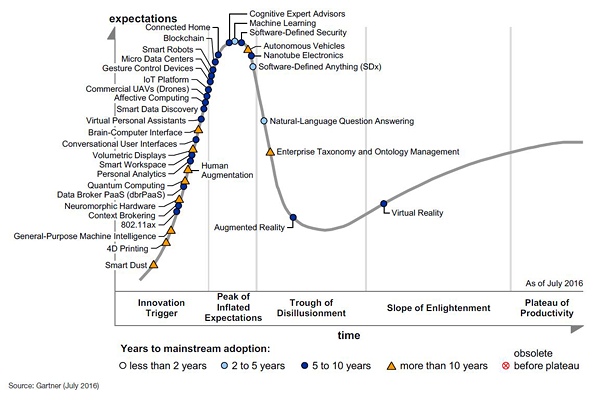
\includegraphics[width=0.75\textwidth]{gartner.png}
\label{gartner}
\caption{\emph{Hype cycle} Gartnera, rok 2016. Poza uczeniem maszynowym znajduje się tu garść technologii opartych o sztuczną inteligencję, m.in \emph{Smart Data Discorvery}, \emph{Natural-Language Question Answering} oraz \emph{General-Purpose Machine Intelligence}}
\end{figure}

Z punktu widzenia analizy danych, uczenie maszynowe jest sposobem na budowę modelu na danych. W istocie klasyfikatory typu bayesowskiego są niczym innym jak praktycznym zastosowaniem reguł prawdopodobieństwa. Zaletą uczenia maszynowego jest automatyczne budowanie hipotezy na danych w przeciwieństwie do klasycznego wnioskowania statystycznego, które wymaga od analityka postawienia hipotez do weryfikacji. \par

"Uczeniem się systemu jest każda autonomiczna zmiana w systemie zachodząca na podstawie doświadczeń, która prowadzi do poprawy jakości jego działania"\cite{cichosz}. Podstawowym celem uczenia maszynowego jest przeprowadzenie \emph{wnioskowania}. Wnioskowanie w rachunku zdań potraktować jako trójkę $ P \wedge W \rightarrow K $, co oznacza, że przesłanki oraz wiedza implikują konkluzję. Wnioskowanie dzieli się na \emph{indukcyjne} i \emph{dedukcyjne}. \par

Wnioskowanie indukcyjne stanowią metody wyciągające ogół ze szczegółu, generalizujące dane do postaci wiedzy. Przykładem jest formowanie reguł podziału na grupy w oparciu o zestaw danych treningowych. Wnioskowanie dedukcyjne stanowi zaaplikowanie wiedzy do określonej sytuacji - w tym wypadku byłoby to użycie tych reguł do nowych danych. \par

W niniejszej pracy przedstawione są dwa z trzech zasadniczych problemów data miningu: klasyfikacja oraz klasteryzacja. Zarówno problem klasyfikacji i klasteryzacji definiuje się w podobny sposób: istotą problemu jest przydzielenie każdego elementu ze skończonego zbioru \emph{obiektów} do jednej lub kilku grup zwanych \emph{kategoriami}. \par

Klasyfikacja może być rozumiana jako uczenie pojęć. Mając zestaw par dane\--ocze\-ki\-wa\-ny wynik, możemy określić tę metodę jako \emph{uczenie z nadzorem}. Celem algorytmu klasyfikujacego jest znalezienie takiej hipotezy, która najlepiej opisuje zależność między przesłanką a konkluzją. W konkretnych zastosowaniach przesłanką jest najczęściej zbiór cech danego obiektu, konkluzją zaś przynależność jego do pewnej klasy obiektów, stąd też nazwa problemu. \par

Grupowanie(clustering) to zadanie tworzenia pojęć bez uprzedniej wiedzy, co klasyfikuje je jako problem \emph{uczenia bez nadzoru}. Możliwe jest rozbicie problemu na dwa zadania: podział na grupy i naukę pojęć. Zazwyczaj realizuje to jedna metoda (kmeans na przykład), jednak można te dwa zadania rozdzielić - wtedy algorytm grupujący generuje dane do algorytmu klasyfikującego.\par

Aby podział na kategorie był satysfakcjonujący, musi spełniać dwa kryteria. Po pierwsze, elementy wewnątrz kategorii muszą być mozliwie do siebie podobne. Po drugie, elementy z różnych kategorii muszą różnić się od siebie o ile jest to tylko możliwe.\par

Aby możliwe było opisanie problemu, potrzebna jest formalne zdefiniowanie zarówno cech, jak i podobieństwa. W praktyce cechy można definiować dwojako: jako wartości binarne lub rzeczywiste (znormalzowane do jedności, lub nie). W ten sposób opis danego obiektu przyjmuje postać wektora cech (ang. \emph{features}). W takiej reprezentacji miarą podobieństwa, lub bardziej niepodobieństwa, jest odległość między tymi dwoma wektorami. Formalnie podobieństwo $s$ między wektorami cech $\vec{x}$ i $\vec{y}$ definiuje się jako:\par

\begin{equation}
s = ( \lvert \vec{x} - \vec{y} \rvert )^{-1}
\end{equation}
\label{similarity}

Ważnym pojęciem do zmierzenia podobieństwa między dwoma obiektami jest pojęcie \emph{metryki}. Metryka jest funkcją, która przyjmując dwa wektory zwraca odległość między nimi. O ile pojęcie odległości pojmowane intuicyjnie jest jednoznaczne, jednak dla celów rozróżnienia obiektów, które są wektorami w przestrzeni o bardzo wielu wymiarach, odpowiednio dobrana metryka pozwala na lepsze dopasowanie modelu klasy do rzeczywistego rozkładu cech wśród jej członków.\par

Najważniejsze dwie metryki to metryka euklidesowa, oraz metryka Manhattan. Są one rozszerzeniem ogólnej metryki Minkowskiego, podanej we wzorze \ref{minkowski}. Szczególnym przypadkiem metryki typu Manhattan jest metryka Hamminga, która dla ciągów binarnych jest analogiem sumą bitów jedynkowych funkcji XOR. \par

\begin{equation}
L_m(\vec{x},\vec{y}) = (\sum\limits_{i=1}^{n} \lvert x_i - y_i \rvert ^m)^{\frac{1}{m}}
\end{equation}
\label{minkowski}

Drugim elementem, poza metryką, definiującym kształt klasy jest \emph{norma}. Norma ma najczęściej postać macierzy $n \times n$ współczynników, gdzie $n$ to długość wektora cech, w której znajdują się współczynniki przekształcające wektor w taki sposób, aby zrównoważyć wpływ różnego rozrzutu cech na klasyfikację, jak i uwzględnić zależności między cechami. Normalizacja wektora $\vec{x}$ przez normę $N$ ma postać podaną we wzorze \ref{norma}. \cite{rutkowski} \par

\begin{equation}
\vec{y} = N \times \vec{x}
\end{equation}
\label{norma}

Uzbrojeni w definicję podobieństwa i sposób jego obliczenia, jesteśmy w stanie w miarę dobrze ocenić poprawność działania algorytmów. Ważnym elementem różnych rozwiązań jest też sposób klasyfikacji: dzieli się ją na \emph{ostrą}, \emph{rozmytą} i \emph{posybilistyczną}. Klasyfikacja ostra przyporządkowuje obiekt do jednej i tylko jednej klasy. Klasyfikacja rozmyta wiąże obiekt z róznymi klasami z różną siłą, przy czym suma współczynników określających przynależność dla danego obiektu jest zawsze równa jedności. Klasifykacja posybilistyczna różni się od poprzedniej zniesieniem ograniczenia sumy.\par


\subsection{Naiwny klasyfikator bayesowski}

Jedna z prostszych metod klasyfikacji opiera się na definicji prawdopodobieństwa warunkowego, zwanej także regułą Bayesa. Stanowi ona związek między prawdopodobieństwami dwóch zmiennych oraz prawdopodobieństwami implikacji jednej zmiennej z drugiej i vice versa. Pozwala ona obliczać prawdopodobieństwo implikacji odwrotnej do implikacji podanej w danych. Reguła ma następującą postać:\par

\begin{equation}
P(C|\vec{x}) = \frac{P(\vec{x}|C)P(C)}{P(\vec{x})}
\end{equation}

Prawdopodobieństwo złożonej zmiennej $\vec{x}$ jest równe iloczynowi prawdopodobieństw jego składowych, jak pokazano we wzorze \ref{pp-zlozone}. Analogicznie można otrzymać prawdopodobieństwo złożonej implikacji \ref{pp-implikacji}. Obydwa wzory funkcjonują na założeniu \emph{niezależności} zmiennych, mianowicie prawdopodobieństwo jednej zmiennej nie jest zależne od żadnej innej. \ref{niezaleznosc}. "Naiwność" klasyfikatora wynika właśnie z założenia niezależności zmiennych, co nie zawsze jest prawdą(wręcz przeciwnie - dla większości sytuacji cechy są ze sobą związane). Uwzględnienie zależności zmiennych pozwala tworzyć kaskadowe modele zwane sieciami bayesowskimi. \cite{dm-cichosz} Nie są one jednak częścią tej pracy.\par

\begin{equation}
P(\vec{x}) = \prod\limits_{i=1}^n{P(x_i)}
\end{equation}
\label{pp-zlozone}

\begin{equation}
P(C|\vec{x}) = \frac{P(C)\prod\limits_{i=1}^n{P(x_i|C)}}{\prod\limits_{i=1}^n{P({x_i})}}
\end{equation}
\label{pp-implikacji}

\begin{equation}
P(A \cap B) = P(A)P(B)
\end{equation}
\label{niezaleznosc}

Naiwny klasifykator bayesowski dla danego wektora wejściowego $\vec{x}$ testuje prawdopodobieństwo każdej z hipotez $P(C_j|\vec{x}) | C_j \in C$, gdzie C to zbiór zdarzeń elementarnych polegających na przynależności elementu do jednej z kategorii. W przypadku klasyfikacji ostrej $\sum\limits_{C_j \in C} P(C_j) = 1 $. Za prawdopodobieństwa zdarzeń elementarnych wchodzących w skład reguły Bayesa przyjmuje się prawdopodobieństwa wystąpienia danych zdarzeń w próbce uczącej. \par

Ze względu na fakt, iż dla nie występującego w próbce uczącej wektora $P(\vec{x}) = 0$ oraz fakt, że $P(\vec{x})=const$ dla każdego $C_j$ człon pomija się, uzywając do klasyfikacji miary proporcjonalnej do prawdopodobieństwa. Następnie jako wynik klasyfikacji przyjmuje się zdarzenie, które osiąga najwyższą miarę.\par
\vspace{0.5cm}
Wady:\par
\begin{itemize}
\item mała akceptowalna ilość hipotez(klasyfikator bierze pod uwagę wszystkie hipotezy i nimi operuje)
\item nieuwzględnienie uporządkowania kategorii (a więc trzeba wstępnie wyznaczyć pojęcia)
\end{itemize}\par
Zalety:\par
\begin{itemize}
\item Niska złożoność obliczeniowa: O(n)
\item Łatwość implementacji
\end{itemize}\par






\subsection{Klasyfikator maksymalnoogległościowy}

Klasyfikatory maksymalnoodległościowe zostały wynalezione przez Vapnika. Opierają się one na wyznaczeniu granicy między zestawmi danych w taki sposób, aby zachować możliwie dużą odległość najbliższych punktów od granicy. Inna nazwa tej metody, \emph{maszyna wektorów wspierających}, oddaje sposób w jaki zostaje to wykonane. Wybiera się $n$ punktów spośród zestawu danych, a następnie wyznacza hiperpowierzchnię dzielącą te punkty. Rycina \ref{hyperplane-png} przedstawia przypadek dla dwóch wymiarów. Sednem algorytmu jest wybranie takich punktów/wektorów, dla których suma odległości od nich do powierzchni jest maksymalna (stąd nazwa). W gruncie rzeczy jest to więc algorytm optymalizacyjny. \par

\begin{figure}
\centering
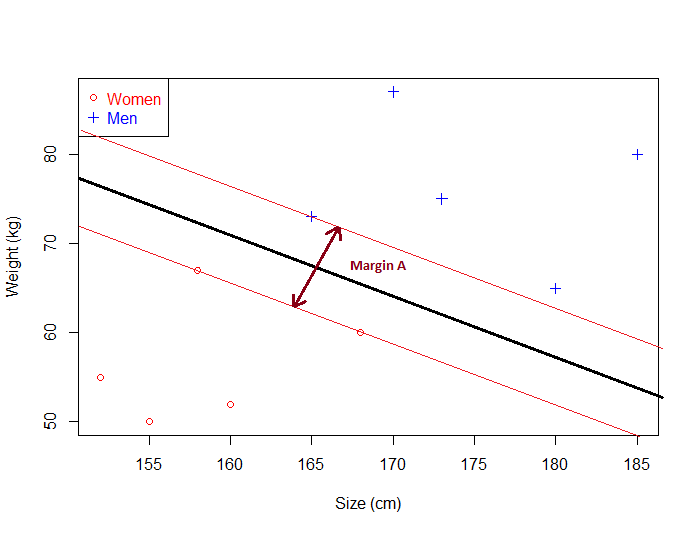
\includegraphics[width=0.8\textwidth]{hyperplane.png}
\label{hyperplane-png}
\caption{Hiperpowierzchnia o maksymalnej odległości. W przypadku dwuwymiarowym o jądrze liniowym ma ona postać prostej o maksymalnej odległości od punktów wspierających.}
\end{figure}


Istotne do poprawnego wykorzystania SVM jest wykonanie kilku kroków \cite{chih-wei}. Po pierwsze, należy przygotować i znormalizować dane. Drugim etapem jest wybór rodzaju funkcji jądra. Standardowo rozróżnia się cztery jej rodzaje: liniowe, wielomianowe, RBF i sigmoidalne. Następnie, należy ocenić odpowiednio wartość zmiennej C, zwanej z angielskiego \emph{penalty variable}. Zgodnie z badaniami samego autora tej metody, musi być ona równa wymiarowi $VC$ (\emph{Vapnika-Chervonenkisa}) dla zbioru danych. Wymiar VC definiuje się w sposób podany we wzorze \ref{wymiar-vc} - mianowicie jest to największa moc zbioru C, który jest w stanie rozbić rodzinę zbiorów H na wszystkie podzbiory C. Wraz z oceną tego parametru należy jeszcze znaleźć współczynnik błędu. \par

\begin{equation}
VC(H) = max(D) \implies \bigvee\limits_C \lvert C \rvert = D \implies H \cap C \supset 2^{C}
\end{equation}
\label{wymiar-vc}

Ze względu na złożoną definicję, wymiar VC jest ciężki do obliczenia, co stanowi jedną z większych przeszkód w wykorzystywaniu SVM. Algorytm ma zaletę, że jest w stanie radzić sobie z zestawami danych, które nie są liniowo-separowalne. W tym celu wykorzystuje się tzw. \emph{kernel trick} - jest to operacja dodania do danych dodatkowej zmiennej, która wiąże określonym wzorem poprzednie zmienne. Odpowiednie związanie zmiennych pozwala sprowadzić zestaw danych do postaci liniowo-separowalnej. \cite{kernel-trick} Ilustracja tego procesu przedstawiona jest na rysunku \ref{kernel-trick-png}

\begin{figure}
\centering
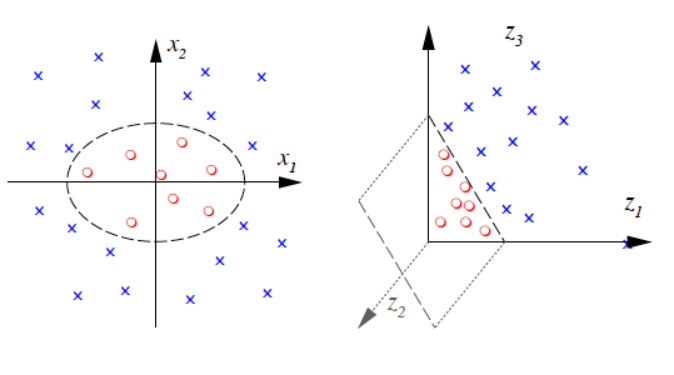
\includegraphics[width=0.8\textwidth]{kernel-trick.png}
\label{kernel-trick-png}
\caption{Przekształcenie zmiennych w celu osiągnięcia liniowej separowalności. Przekształcone zmienne (lub podzbiór zmiennych) dołączane są do zestawu danych. Na rysunku przedstawione jest osiągnięcie liniowej separowalności poprzez zamianę układu współrzędnych na układ biegunowy.}
\end{figure}\par
\vspace{0.5cm}
Wady:\par
\begin{itemize}
\item Duża złożoność obliczeniowa (pomiędzy $O(n^2)$ a $O(n^3)$)
\end{itemize}\par
Zalety:\par
\begin{itemize}
\item Możliwość separacji danych nieseparowalnych liniowo
\item Możliwość wykorzystania w budowaniu modelu regresyjnego
\end{itemize}\par

\subsection{Metoda k średnich}

Metoda k-średnich stanowi niewątpliwie jeden z najprostszych algorytmów klastrujących. Jej działanie opiera się na iteracyjnym grupowaniu i klasyfikowaniu elementów. Jego działanie najlepiej przedstawione jest na rysunku \ref{kmeans-png}. Cykl poprawiania średnich trwa aż ich zmiana będzie mniejsza od progu.\par

\begin{figure}
\centering
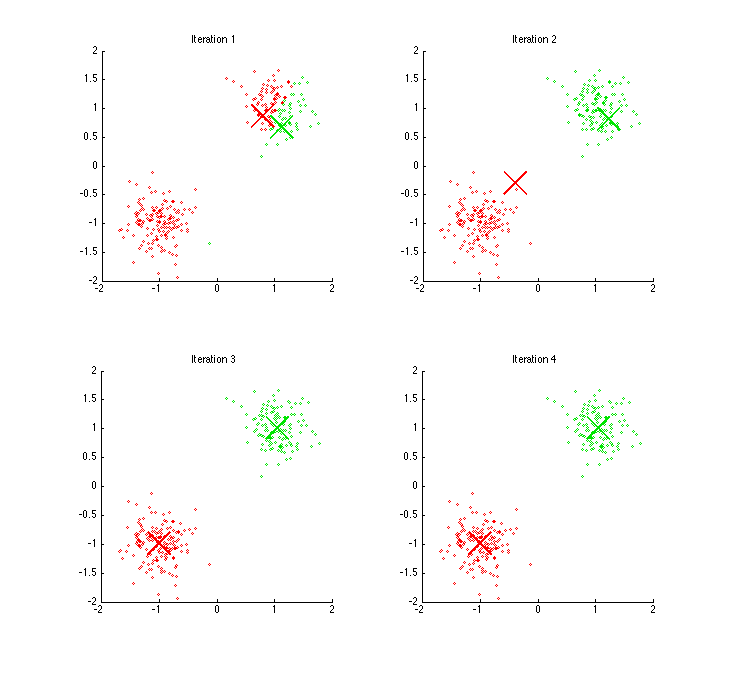
\includegraphics[width=0.8\textwidth]{kmeans.png}
\label{kmeans-png}
\caption{Ilustracja działania metody k-średnich. Początkowo losowo rozmieszczone centra są iteracyjnie przyciągane w taki sposób, aby możliwie dokładnie odwzorować występujące grupy. Należy zwrócić uwagę na rozdzielenie bardzo blisko położonych centr w pierwszej iteracji.}
\end{figure}

Metodę k-średnich można wykorzystać do klasyfikacji danych na podstawie otrzymanego modelu. Klasyfikacja ta ma charakter minimalnoodległościowy - obiekt przynależy do grupy, do której środka ciężkości ma najbliżej. Nie jest to jednak efektywna metoda klasyfikacji, a wykorzystanie tej metody do przypisania do już istniejących cech wiąże się z rozwiązaniem problemu rozbieżności etykiet nadanych przez klasyfikator i rzeczywiście opisujących zestaw danych. Z tego powodu, jako metoda klastryzacji, jest ona bardziej użyteczna jako metoda eksploracyjna. \par
\vspace{0.5cm}
Wady:\par
\begin{itemize}
\item Odgórnie ustalona liczba kategorii
\item Mała odporność na liniowo-nieseparowalne grupy
\item NP-złożoność
\end{itemize}\par
Zalety:\par
\begin{itemize}
\item Prostota implementacji
\end{itemize}\par



\section{Walidacja krzyżowa}

Sprawdzenie skuteczności klasyfikacji przez dany model przeprowadza się metodą walidacji krzyżowej. Polega ona na podziale próbki na zestaw danych uczących i walidujących. Podział ma charakter losowy. Model uczony na pierwszym zestawie następnie klasyfikuje obiekty z drugiego zestawu. Wynik tej klasyfikacji jest porównywany z poprawnymi etykietami zawartymi w zestawie danych. Kilkukrotne przeprowadzenie takiej walidacji pozwala lepiej przybliżyć dokładność klasyfikatora.\par

Błąd próbki dany jest przez wzór \ref{bp}. Analogicznie do błędu rzeczywistego (\ref{br}) jest to ilość niepoprawnych klasyfikacji w stosunku do wszystkich wektorów cech - dla próbki w tejże próbce, dla rzeczywistego w przestrzeni wszystkich mozliwych wektorów cech. Liczba pomyłek dana jest przez \ref{lp}. W podanym wzorze możemy przypisać $\Omega$ jako jednorodny rozkład spośród próbki danych weryfikacyjnych.


\begin{equation}
e_P^c(h) = \frac{| \{ x \in P | h(x) != c(x) \} |}{|P|}
\end{equation}
\label{bp}

\begin{equation}
e_\Omega^c (h) = Pr_{x \in \Omega}(h(x) != c(x))
\end{equation}
\label{br}

\begin{equation}
r_P^c(h) = | \{ x \in P | h(x) != c(x) \} | 
\end{equation}
\label{lp}

\chapter{Opis wykorzystanego kwestionariusza}

Do zrealizowania systemu wybrano ogólnodostępny zestaw danych psychologicznych, pobrany ze strony internetowej \cite{raw_data}. Dane zawierają wyniki testu przeprowadzonego w Internecie wraz z metryczką demograficzną. Test składa się z 48 pytań w pięciostopniowej skali Likerta.\par

\section{Model Hollanda}

Model ten opracowany przez John'a Hollanda w roku 1959. \cite{holland-source} Klasyfikuje on ludzi na sześć głównych klas, a bardziej szczegółowo, szereguje funkcje zawodowe ludzi według ich preferencji. Te sześć funkcji zestawionych jest w przeciwstawne pary:\par

\begin{itemize}
\item Artystyczny - Konwencjonalny (A-C)
\item Realistyczny - Społeczny (R-S)
\item Badawczy - Przedsiębiorczy (I-E)
\end{itemize}

Przeciwstawność tych atutów wynika z ich definicji: typ realistyczny skupiony jest na zadaniach, podczas gdy typ społeczny skupia się na materii międzyludzkiej; analogicznie artysta lubuje się w odkrywaniu, podczas gdy typ konwencjonalny lubi pracę jasno zdefiniowaną i powtarzalną. Najmniej oczywista jest dychotomia między typem badawczym a przedsiębiorczym. Analiza danych pobranych w wyżej wspomnianego źródła wskazuje na najmniejszą korelację dla wszystkich tych trzech par, z negatywną korelacją dla pary A-C.\par

Zawody są przydzielone do jednej lub kilku z tych klas według umiejętności, których wymagają, mogą one należeć także do klas przeciwstawnych, jeżeli obydwie umiejętności są potrzebne - nie wykluczają się one wzajemnie. Listy zawodów względem preferencji są ogólnie dostępne w internecie, co wpływa na użyteczność testu Hollanda. \par

\section{Skala Likerta}

Skala Likerta jest techniką psychometryczną używaną w celu zmierzenia stopnia zgodności respondenta z danym poglądem lub podejściem. Skala ta najczęściej jest jednowymiarowa. Składa się z małej ilości odpowiedzi przedstawiąjach symetrycznie ułożone punkty na osi \emph{zgodność}-\emph{niezgodność}, w nieparzystej ilości(zazwyczaj 5). Parzysta ilość jest czasami wprowadzona celem usunięcia możliwości zajęcia stanowiska neutralnego. \par

Założenie, że punkty przedstawiają równoodległe natężenia cechy, pozwala traktować skalę jako źródło danych interwałowych. Dane interwałowe oddają różnice między różnymi poziomami danej cechy, nie określają jednak jej absolutnej wartości (punktu zerowego). \cite{bertram} Można więc na nich wyznaczać odległości, co jest podstawą do definiowania podobieństwa według definicji \ref{similarity}.\par

Analiza wyników testu opartego na tej skali zależy od sposobu ujęcia odpowiedzi. Jeżeli analizujemy pojedyńcze zdania, danych nie można traktować jako danych interwałowych i stosuje się wtedy techniki nieparametryczne. Natomiast wziąwszy zestawy odpowiedzi opisujące poszczególną cechę, można potraktować tę technikę jako metodę ilościową i stosować metody statystyki parametrycznej. \cite{joe} Z tego też powodu skala Likerta zwana jest także techniką sumacyjną. \par

W niniejszej pracy skala jest potraktowana nieco bardziej liberalnie: traktuje się poszczególne cechy jako niezależne zmienne o charakterze interwałowym. O ile jest to niepoprawne z punktu widzenia pojedyńczego pomiaru, dla dużej populacji można zastosować to przybliżenie. \par




\chapter{Implementacja}

W ramach pracy zbudowany został system pozwalający przeprowadzać testy na podstawie kwestionariuszy, przeprowadzać klasyfikację respondentów na podstawie odpowiedzi i analizować zebrane dane. Aplikacja została napisana w języku Python, który jest szeroko wykorzystywany w środowiskach analitycznych. Wykorzystano wersję języka o numerze 2.7.\par

Front-end aplikacji, który stanowi także jej szkielet, napisano przy pomocy pakietu \emph{Flask}. Jest to open-source'owy lekki serwer HTTP, wykorzystujący język pomocniczy \emph{Jinja2} do generacji dokumentów HTML przy pomocy danych z aplikacji. Mechanizm ten użyty został do wstrzykiwania danych testu do prostej aplikacji sieciowej opartej o \emph{Javascript}. Użytkownik może wybrać test na stronie głównej, można też udostępniać testy jedynie przy pomocy statycznych linków.\par

Test generowany przez aplikację może zawierać pytania o charakterze binarnym, jak i przy użyciu skali Likerta. Podczas przebiegu testu ukazywane jest tylko jedno pytanie na raz, co pozwala skupić się na odpowiedzi. Wyniki są zbierane dopiero w przypadku ukończenia testu. Po zakończonym teście użytkownik jest przekierowywany na stronę, na której może udostępnić dodatkowe informacje w celach analityki. Po przejściu tego etapu wyświetlany jest raport z testu.\par

Generacja raportów oparta jest o pakiety \emph{pandas} oraz \emph{matplotlib}. Użycie tych dwóch bibliotek pozwala na używanie najpowszechniejszych metod analityki na zestawach danych, włącznie z generowaniem wykresów. Struktura raportów oparta jest o definicje w plikach konfiguracyjnych poszczególnych testów(o których później). Zawierają one definicje raportów zbudowane przy użyciu struktury przypominającej struktury języka LISP, używające składni JSON. Wywołania tego języka przedstawiono w tabeli \ref{lang}.\par

\begin{table}
\begin{tabular}{l|l|l}
\hline
Komenda & Argumenty & Opis \\
log            & str  repl... & Loguje do konsoli, wstawiając repl \\
print          & str  repl... & J.w. ale zwraca HTML \\
safePrint      & str  repl... & J.w. ale zwraca tekst(można stosować tagi HTML)\\
\$...          & value & Przypisz do zmiennej\\
df             & & Specjalna zmienna - podany dataset/wektor cech\\
get            & ix var & Pobierz element ix ze zmiennej\\
set            & ix var & Pobierz element ix ze zmiennej \\
split          & ratio   data & Dzieli dataset losowo na dwa o odp. proporcjach \\
fit            & model   labelcol     data & Trenuje nowy model na podanych danych \\
score          & model   data & Oceń model uzywając podanego zestawu danych\\
predict        & model   list & Zastosuj model do danego wektora cech\\
select         & data cols... & Wybierz tylko kolumny\\
drop           & data cols... & Wybierz wszystkie kolumny bez podanych\\
describe       & data & Podaj podstawowe cechy statystyczne zestawu danych\\
corr           & data & Podaj korelację zestawu danych\\
map            & data expr... & Stwórz nowe kolumny z wyrażeń typu "nazwa = wyrażenie"\\
query          & data query & Przefiltruj zestaw danych po rekordach\\
aggreg         & list aggregations... & Stwórz listę z nowych danych\\
+              & indices... & Argument do aggreg, sumuje kolumny o podanych indeksach\\
bar            & data & Wykres słupkowy \\
\hline
\end{tabular}
\caption{Komendy do budowy raportów}
\label{lang}
\end{table}

Metody klasyfikacji oraz uczenia maszynowego pochodzą z biblioteki \emph{sklearn}. Są one udostępniane jako dyrektywy do języka konfiguracyjnego. Istnieje możliwość nauczenia klasyfikatorów w trakcie uruchamiania aplikacji, jak i ich dynamiczne zastępowanie nowymi w trakcie działania aplikacji. Wykorzystane techniki obejmują: klasifykator Bayesowski, metodę k-średnich oraz maszynę wektorów wspierających.\par

Aplikacja udostępnia widok, który generuje raporty dla całego zestawu danych. Raporty te mogą korzystać z danych wzorcowych jak i zebranych podczas testowania. Funkcja ta ma na celu umożliwienie przeprowadzenia analizy danych, zarówno wstępnej jak i weryfikacyjnej, która z kolei umożliwi dopracowanie modelu.\par

Front-end udostępnia także widok interaktywny do budowania raportów z danych bez wcześniejszego definiowania ich. Użyty jest ten sam język, co w plikach konfiguracji raportów. Pozwala to na sprawdzanie hipotez bez konieczności rebootowania aplikacji.\par

\section{Pliki konfiguracyjne}

Pliki konfiguracyjne do programu oparte są o standard JSON. Pozwala to na łatwe wbudowanie złożonych ustawień takich jak sekwencje wykonywanych operacji podczas generowania odpowiedzi na test czy precyzowanie pytań o różnej strukturze.\par

Głównym plikiem konfiguracyjnym jest \texttt{static/tests.json}. W nim zawarte są informacje dotyczące: zestawu pytań, lokalizacji logów i danych odniesienia, dodatkowych parametrów testu oraz metod generacji raportów. Kompletną listę dyrektyw zestawiono w tabeli \ref{lang}. Drugim typem plików konfiguracyjnych są pliki linkowane przez poszczególne testy. Struktura takiego pliku to lista obiektów przedstawiających pytania do testów.\par

Schemy tych dwóch rodzajów plików przedstawione są w tabelach \ref{tests-schema} i \ref{questions-schema}

\section{Instalacja i uruchomienie}

Całość programu zaopatrzono w skrypty instalacyjne do generacji niezależnego środowiska Pythona \emph{virtualenv}. Skrypty instalacyjne testowane były na środowisku Ubuntu LTS oraz Linux Mint - obydwa te systemy oparte są o dystrybucję Debian i menedżer pakietów \emph{apt-get}. Uruchomienie na innym systemie Linux wymaga dostosowania menedzera pakietów. Instalacja pod innymi systemami nie była uwzględniana ze wzgledu na mozliwość uruchomienia aplikacji w chmurze.  Kod źródłowy wraz z tekstem tej pracy i notatkami udostępniono poprzez serwis github: \emph{https://github.com/Zantyr/dissertation}\par

\chapter{Wyniki analiz i przedstawienie działania aplikacji}



\section{Wyniki EDA}

Na zestawie danych przeprowadzono wstępną analizę danych. Ze względu na jej długość nie załączono jej w treść rozdziału, a dołączono jako dodatek do pracy razem z listingiem kodu. W niniejszym rozdziale zamieszczono jedynie streszczony przebieg analizy. \par

Zestaw danych oczyszczono, a następnie stworzono z niego dwa inne: jeden zawierający dane zagregowane względem krajów, drugi, na którym przeprowadzono analizę rozkładu wieku wśród responentów.  Na podstawie tego przeglądu stworzono pięć zestawów danych: \par

\begin{itemize}
\item próbka losowa
\item kraje europejskie o identycznej preferencji co Polska
\item kraje europejskie o równych płciach
\item próbka losowa z wyborem cech
\item próbka losowa z etykietami z algorytmu klastryzacji
\end{itemize}

Dla każdego z zestawów danych wykonano autokorelację celem sprawdzenia poprawności danych, której wyniki przedstawiono w tabeli \ref{autokorelacja}. Ze względu na duży rozrzut ilości cech reprezentujących dane kategorie w zestawie o wybranych cechach, zrezygnowano z preprowadzenia autokorelacji. Zapisano zestawy po pięćset rekordów wybranych losowo z każdego zestawu danych. Każdy taki plik został następnie wykorzystany do konstrukcji odrębnego klasyfikatora, bazowanego na jednym z dwóch algorytmów: SVM lub Naive Bayes.\par

\begin{table}
\begin{tabular}{l|l|l|l|l|l|l}
\hline
 & R & I & A & S & E & C \\
R & 1.000000 & 0.351583 & 0.116827 & 0.053365 & 0.222281 & 0.460326 \\
I & 0.351583 & 1.000000 & 0.293377 & 0.173280 & 0.075742 & 0.142551 \\
A & 0.116827 & 0.293377 & 1.000000 & 0.298863 & 0.225001 & -0.062294 \\
S & 0.053365 & 0.173280 & 0.298863 & 1.000000 & 0.420071 & 0.170134 \\
E & 0.222281 & 0.075742 & 0.225001 & 0.420071 & 1.000000 & 0.499153 \\
C & 0.460326 & 0.142551 & -0.062294 & 0.170134 & 0.499153 & 1.000000 \\
\hline
 & R & I & A & S & E & C \\
R & 1.000000 & 0.392197 & 0.093335 & 0.080263 & 0.215052 & 0.476342 \\
I & 0.392197 & 1.000000 & 0.341903 & 0.204322 & 0.031996 & 0.130974 \\
A & 0.093335 & 0.341903 & 1.000000 & 0.367359 & 0.196295 & -0.096838 \\
S & 0.080263 & 0.204322 & 0.367359 & 1.000000 & 0.347138 & 0.062591 \\
E & 0.215052 & 0.031996 & 0.196295 & 0.347138 & 1.000000 & 0.428114 \\
C & 0.476342 & 0.130974 & -0.096838 & 0.062591 & 0.428114 & 1.000000 \\
\hline
 & R & I & A & S & E & C \\
R & 1.000000 & 0.330095 & 0.114161 & 0.022075 & 0.244910 & 0.447003 \\
I & 0.330095 & 1.000000 & 0.311654 & 0.139892 & 0.043397 & 0.112865 \\
A & 0.114161 & 0.311654 & 1.000000 & 0.292624 & 0.224672 & -0.081070 \\
S & 0.022075 & 0.139892 & 0.292624 & 1.000000 & 0.406622 & 0.128495 \\
E & 0.244910 & 0.043397 & 0.224672 & 0.406622 & 1.000000 & 0.443659 \\
C & 0.447003 & 0.112865 & -0.081070 & 0.128495 & 0.443659 & 1.000000 \\
\hline
 & R & I & A & S & E & C \\ 
R & 1.000000 & 0.331143 & 0.119409 & 0.051537 & 0.249179 & 0.463329 \\ 
I & 0.331143 & 1.000000 & 0.314317 & 0.148906 & 0.021750 & 0.099953 \\ 
A & 0.119409 & 0.314317 & 1.000000 & 0.301875 & 0.225229 & -0.075600 \\ 
S & 0.051537 & 0.148906 & 0.301875 & 1.000000 & 0.395553 & 0.134766 \\ 
E & 0.249179 & 0.021750 & 0.225229 & 0.395553 & 1.000000 & 0.446287 \\ 
C & 0.463329 & 0.099953 & -0.075600 & 0.134766 & 0.446287 & 1.000000 \\ 
\hline
\end{tabular}
\caption{Autokorelacje zestawów danych, kolejno: losowej próbki, identycznej preferencji i równomiernej płci}
\label{autokorelacja}
\end{table}


Planowano także stworzyć zestaw danych o profilu wiekowym identycznym do polskiego, jednak pomysł zarzucono po ustaleniu, że próbka nie jest reprezentacyjna (zaledwie dziewięć rekordów z podanym wiekiem). Stworzono jednak histogramy dla całego zestawu danych i załączono je w \ref{histo1} i \ref{histo2}. \par

\begin{figure}
\centering
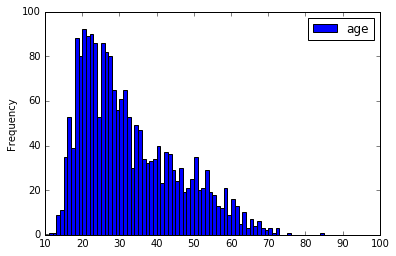
\includegraphics[width=0.8\textwidth]{histo1.png}
\label{histo1}
\caption{Histogram dla danych z podanym wiekiem. Należy zauważyć mocne scentrowanie danych wokół ludzi młodych, przeważnie w wieku poszukiwania pierwszego zawodu.}
\end{figure}

\begin{figure}
\centering
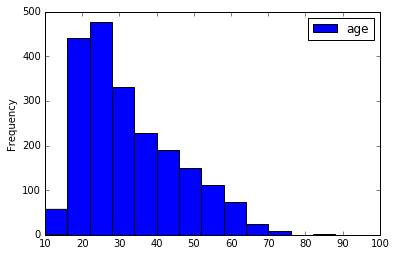
\includegraphics[width=0.8\textwidth]{histo2.png}
\label{histo2}
\caption{Histogram dla danych z wiekiem w przedziałach po 6 lat. Wnioski analogiczne, jak w poprzednim histogramie - przeważają ludzie bez lub z małym doświadczeniem zawodowym.}
\end{figure}


Wykonano także wykresy radarowe dla poszczególnych grup wiekowych, celem porównania zmieniających się z wiekiem/czasem 
preferencji zawodowych oraz zróżnicowania płciowego. Przedstawiono wyniki na rysunku \ref{profile} \par

\begin{figure}
\centering
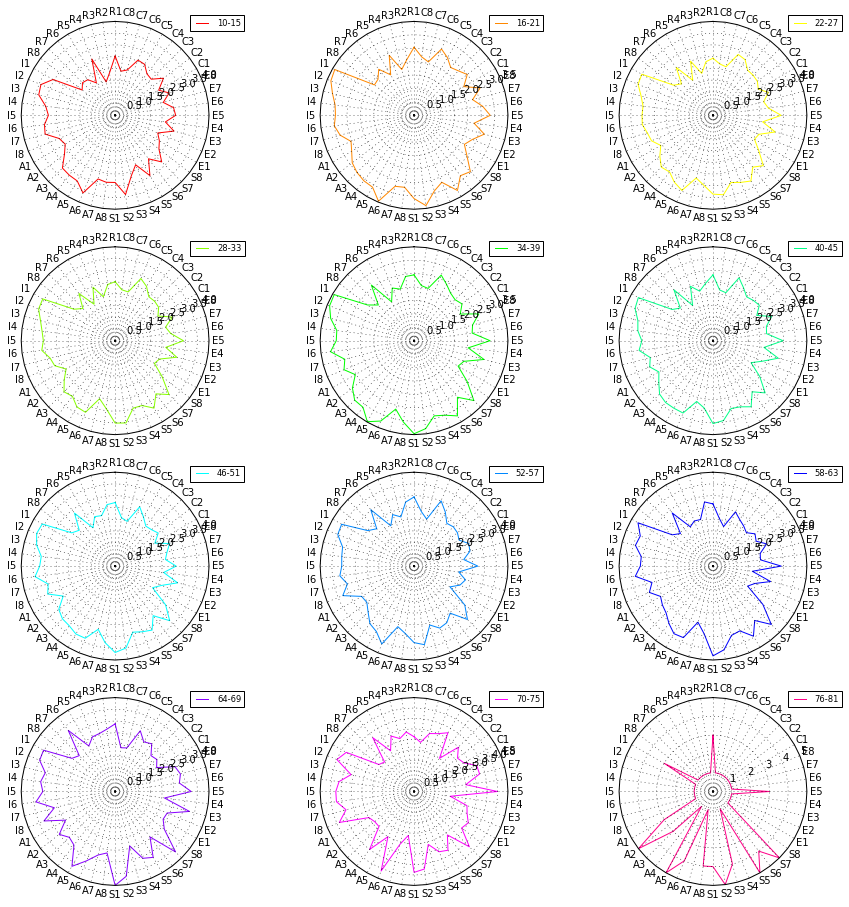
\includegraphics[width=1\textwidth]{profile.png}
\label{profile}
\caption{Profile dla grup wiekowych. Na większości wykresów widoczna jest wyraźna tendencja do uprawiania zawodów z grup Intelektualnej, Artystycznej i Społecznej. Na uwagę zasługuje ostatni diagram, na którym przedstawiony został profil pojedyńczego odpowiadającego.}
\end{figure}

\section{Działanie aplikacji}

Aplikacja ładuje dowolną testów umieszczonych w plikach konfiguracyjnych i udostępnia je w widoku głównym (\ref{main-menu}). Wybrany test prezentuje jedno pytanie jednocześnie, przy czym możliwe są pytania w skali Likerta oraz typu \emph{tak-nie} \ref{questions}. Pytania nie są zapisywane w trakcie sesji. Kliknięcie na przycisk z pytaniem resetuje przebieg testu.  Po wykonaniu testu użytkownik zostaje przekierowany do strony, na której może podać dodatkowe informacje do logowania \ref{additional-info}. Następnie prezentowane są mu wyniki, generowane według określonego skryptu raportu. W przedstawionej wersji są to wyniki numeryczne. Do raportu z wynikami można dołączyć dowolną ilość wykresów. (\ref{outputs}). \par

Pod URL \texttt{/report/<id>} generowany jest raport dotyczący całych zebranych danych, oprogramowany analogicznie do raportu wynikowego. W przedstawionej implementacji jest to raport prezentujący wyniki walidacji krzyżowej, która przeprowadzana jest podczas uruchamiania serwera. Pod URL \texttt{/console/<id>} prezentowana jest konsola, w której można testować wywołania języka skryptowego.\par

\begin{figure}
\centering
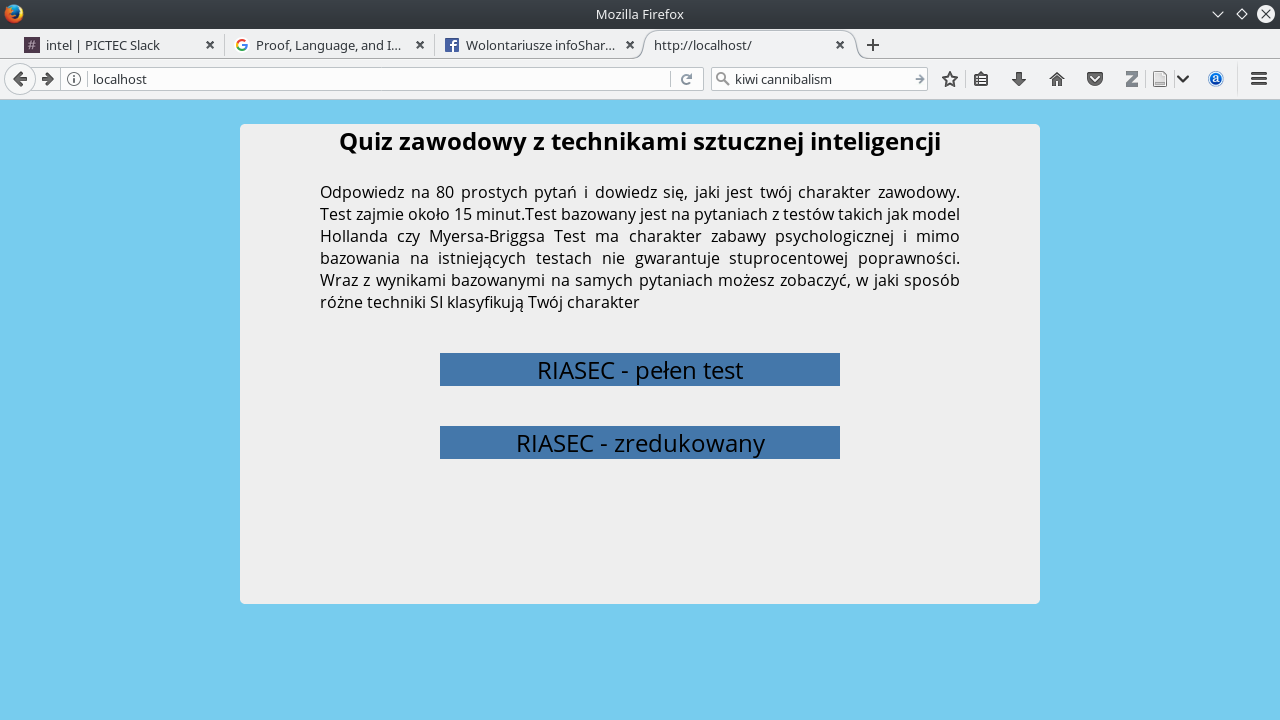
\includegraphics[width=0.8\textwidth]{4.png}
\label{main-menu}
\caption{Menu wyboru testu}
\end{figure}

\begin{figure}
\centering
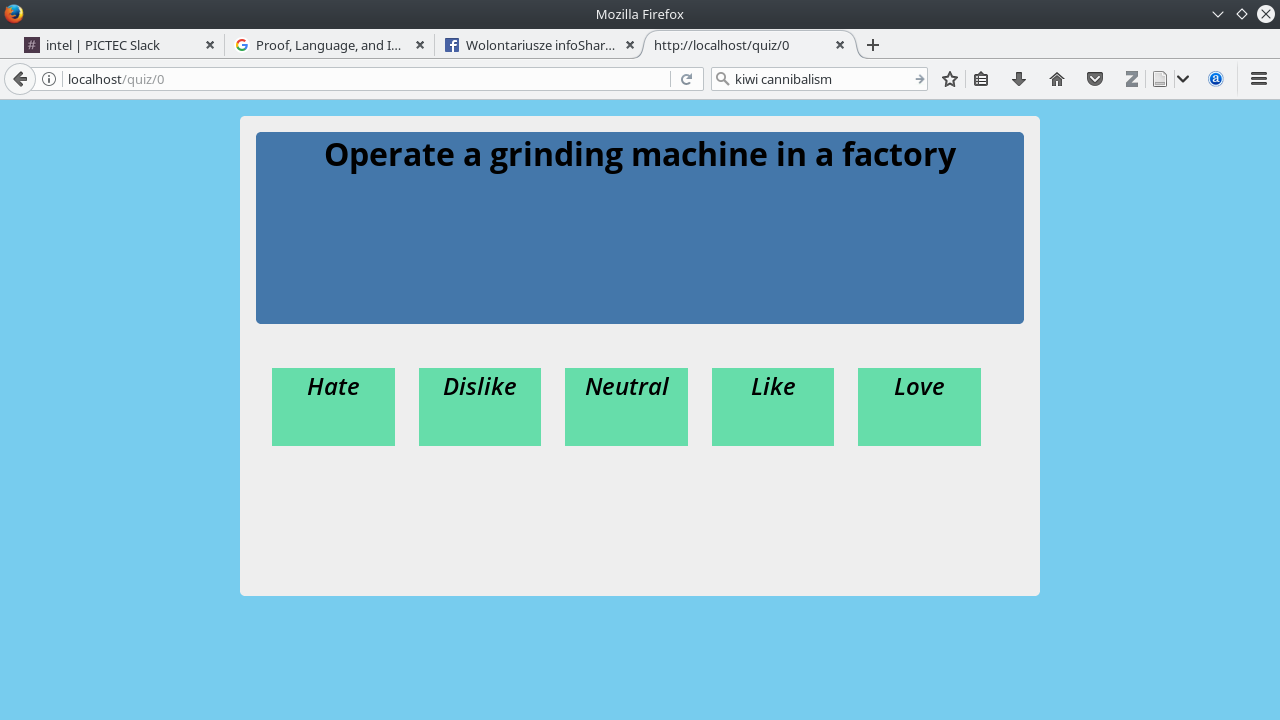
\includegraphics[width=0.8\textwidth]{2.png}
\label{questions}
\caption{Pytanie ze skalą Likerta}
\end{figure}

\begin{figure}
\centering
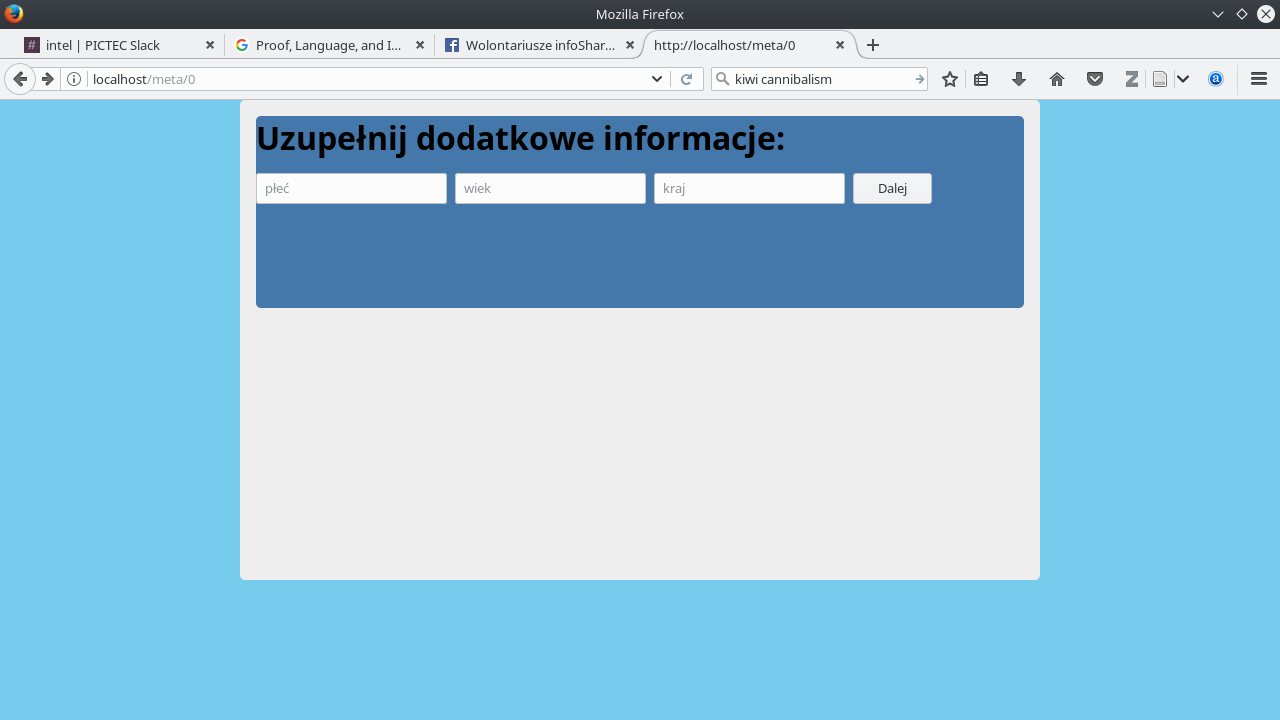
\includegraphics[width=0.8\textwidth]{3.png}
\label{additional-info}
\caption{Zapytanie o dodatkowe informacje}
\end{figure}

\begin{figure}
\centering
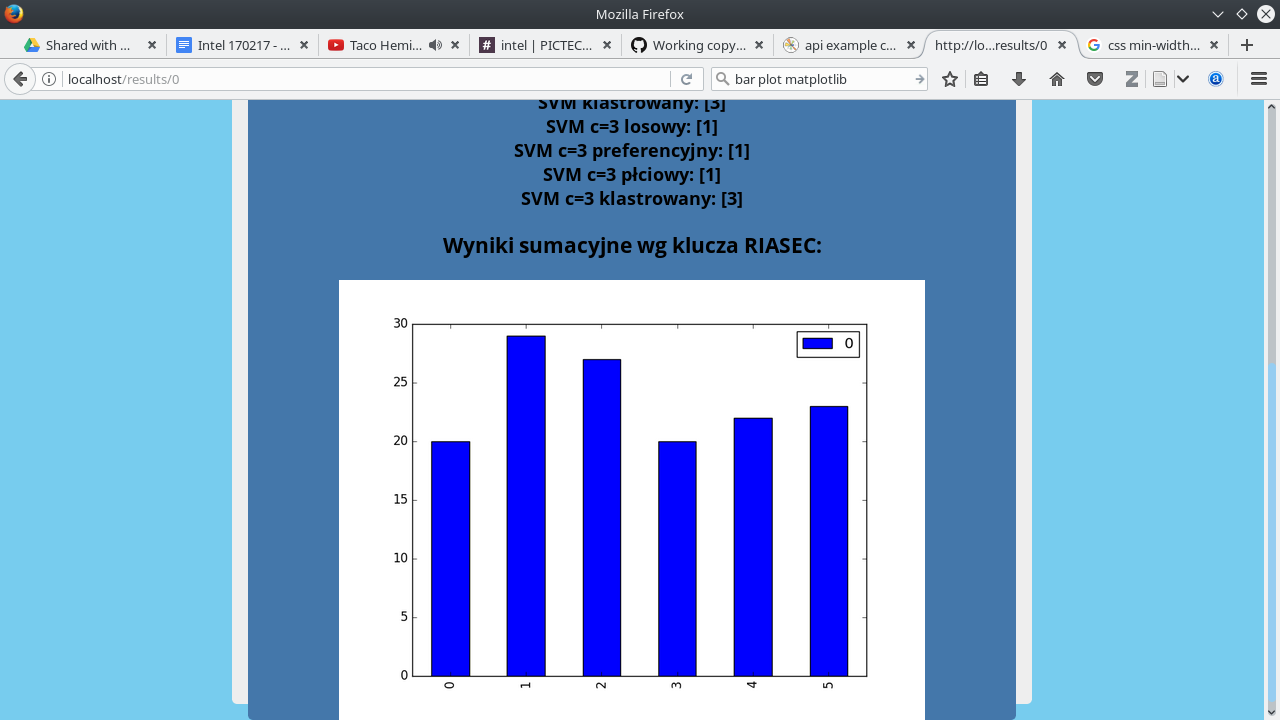
\includegraphics[width=0.8\textwidth]{10.png}
\label{outputs}
\caption{Wykres wynikowy}
\end{figure}

\section{Porównanie trafności klasyfikatorów}

Skonfigurowano aplikację, aby przeprowadzała walidację krzyżową na próbkach po ich klasyfikacji. Wyniki walidacji wyświetlono w raporcie do wyników testu, (rysunek \ref{cross-validation}). Ze względu na losowy dobór próbki, wyniki mogą się różnić między uruchomieniami. W tabeli \ref{cross-val-tab} przedstawiono wyniki dziesięciu kolejnych walidacji. Uśrednione wyniki znajdują się w tabeli \ref{cross-val-tab-av}.

\begin{figure}
\centering
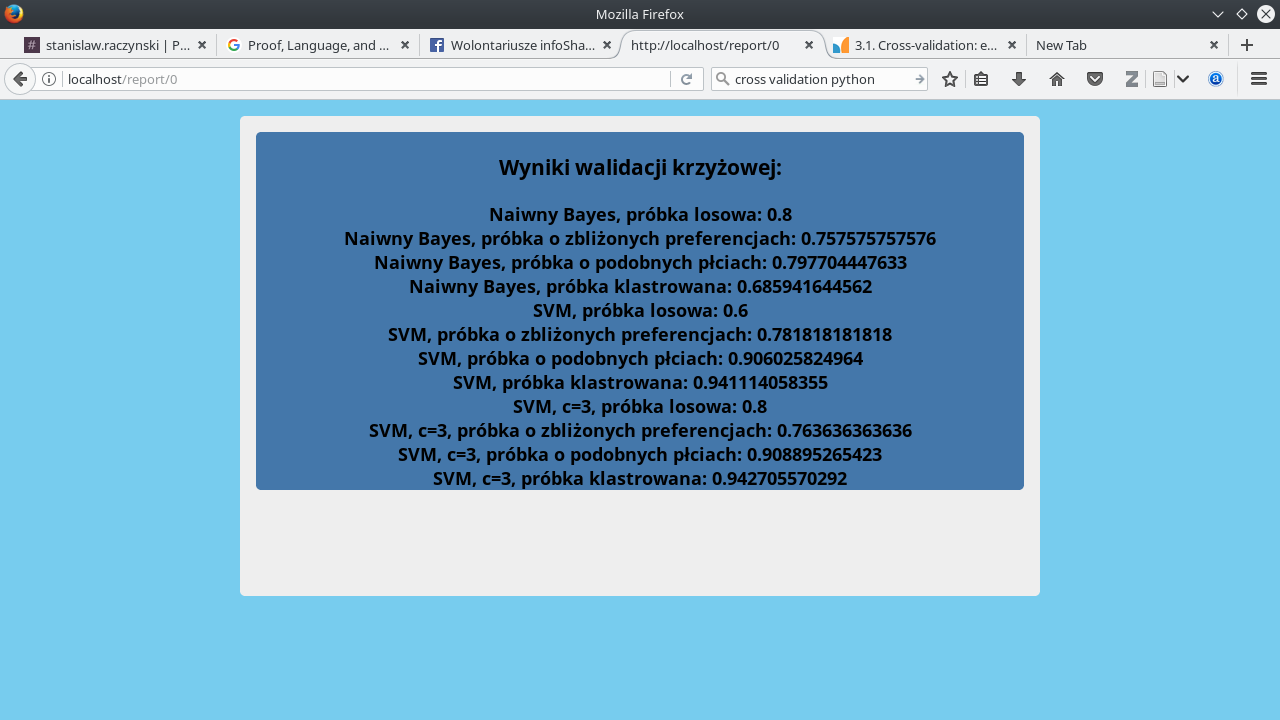
\includegraphics[width=0.8\textwidth]{5.png}
\label{cross-validation}
\caption{Raport z wynikami walidacji krzyżowej}
\end{figure}

\begin{table}
\begin{tabular}{l|l|l|l|l|l|l|l|l|l|l}
\hline
{\small Bayes, pr. losowa:                     } & {\small 0.66 } & {\small 0.75 } & {\small 0.72 } & {\small 0.66 } & {\small 0.75 } & {\small 0.69 } & {\small 0.75 } & {\small 0.77 } & {\small 0.73 } & {\small 0.71 } \\ 
{\small Bayes, preferencje: } & {\small 0.81 } & {\small 0.73 } & {\small 0.80 } & {\small 0.73 } & {\small 0.74 } & {\small 0.70 } & {\small 0.82 } & {\small 0.72 } & {\small 0.75 } & 0.72 \\
{\small Bayes, równe płcie:        } & {\small 0.72 } & {\small 0.76 } & {\small 0.8 } & {\small 0.75 } & {\small 0.77 } & {\small 0.86 } & {\small 0.83 } & {\small 0.79 } & {\small 0.80 } & {\small 0.85 } \\ 
{\small Bayes, pr. klastrowana:                } & {\small 0.67 } & {\small 0.66 } & {\small 0.69 } & {\small 0.63 } & {\small 0.66 } & {\small 0.71 } & {\small 0.65 } & {\small 0.65 } & {\small 0.72 } & 0.68 \\
{\small SVM, pr. losowa:                              } & {\small 0.71 } & {\small 0.78 } & {\small 0.83 } & {\small 0.68 } & {\small 0.75 } & {\small 0.74 } & {\small 0.78 } & {\small 0.73 } & {\small 0.76 } & 0.75 \\
{\small SVM, preferencje:          } & {\small 0.79 } & {\small 0.75 } & {\small 0.72 } & {\small 0.76 } & {\small 0.74 } & {\small 0.77 } & {\small 0.75 } & {\small 0.80 } & {\small 0.73 } & 0.80 \\
{\small SVM, równe płcie:                 } & {\small 0.8 } & {\small 0.76 } & {\small 0.73 } & {\small 0.77 } & {\small 0.85 } & {\small 0.82 } & {\small 0.78 } & {\small 0.78 } & {\small 0.78 } & 0.80 \\
{\small SVM, pr. klastrowana:                         } & {\small 0.9 } & {\small 0.88 } & {\small 0.90 } & {\small 0.87 } & {\small 0.87 } & {\small 0.88 } & {\small 0.92 } & {\small 0.90 } & {\small 0.92 } & {\small 0.86 } \\ 
{\small SVM $C=3$, pr. losowa: } & {\small 0.72 } & {\small 0.80 } & {\small 0.82 } & {\small 0.70 } & {\small 0.78 } & {\small 0.75 } & {\small 0.78 } & {\small 0.75 } & {\small 0.78 } & {\small 0.76 } \\ 
{\small SVM $C=3$, preferencje: } & {\small 0.76 } & {\small 0.77 } & {\small 0.73 } & {\small 0.75 } & {\small 0.78 } & {\small 0.79 } & {\small 0.73 } & {\small 0.85 } & {\small 0.79 } & {\small 0.81 } \\ 
{\small SVM $C=3$, równe płcie: } & {\small 0.80 } & {\small 0.76 } & {\small 0.76 } & {\small 0.78 } & {\small 0.84 } & {\small 0.84 } & {\small 0.79 } & {\small 0.79 } & {\small 0.79 } & {\small 0.80 } \\ 
{\small SVM $C=3$, pr. klastrowana: } & {\small 0.91 } & {\small 0.88 } & {\small 0.92 } & {\small 0.87 } & {\small 0.87 } & {\small 0.88 } & {\small 0.92 } & {\small 0.90 } & {\small 0.91 } & {\small 0.86 } \\ 


\hline
\end{tabular}
\caption{Wyniki kolejnych walidacji krzyżowych}
\label{cross-val-tab}
\end{table}

\begin{table}
\begin{tabular}{l|l|l|l|l|l|l|l|l|l|l|l}
\hline
NB1 & NB2 & NB3 & NB4 & SV1 & SV2 & SV3 & SV4 & SC1 & SC2 & SC 3 & SC4 \\
    0.724 & 0.757 & 0.797 & 0.676 & 0.754 & 0.765 & 0.791 & 0.894 & 0.767 & 0.781 & 0.800 & 0.896 \\
\hline
\end{tabular}
\caption{Uśrednione wyniki walidacji krzyżowych}
\label{cross-val-tab-av}
\end{table}

W tabeli \ref{sample-out} zestawiono przykładowe wyniki klasyfikacji. Widoczna jest duża zgodność między klasyfikatorami typu SVM dla odpowiadających sobie typów. Należy zauważyć, że klasyfikatory trenowane na zestawie danych nr 4 mają własne oznaczenia numeryczne i są między sobą zgodne.

\begin{table}
\begin{tabular}{l|l|l|l|l|l|l|l|l|l|l|l|l}
\hline
NB1 & NB2 & NB3 & NB4 & SV1 & SV2 & SV3 & SV4 & SC1 & SC2 & SC 3 & SC4 & Likert \\
2 & 2 & 2 & 1 & 2 & 2 & 2 & 5 & 2 & 2 & 2 & 5 & 2 \\ 
4 & 4 & 4 & 0 & 2 & 4 & 4 & 0 & 2 & 4 & 4 & 0 & 4 \\ 
0 & 0 & 0 & 3 & 3 & 3 & 1 & 3 & 3 & 3 & 1 & 3 & 0 \\ 
2 & 2 & 2 & 1 & 3 & 2 & 1 & 2 & 3 & 2 & 1 & 2 & 1/2/3(fake data) \\ 
2 & 1 & 1 & 3 & 2 & 1 & 2 & 3 & 2 & 1 & 2 & 3 & 2 \\ 
\hline
\end{tabular}
\caption{Przykładowe wyniki klasyfikacji}
\label{sample-out}
\end{table}

\section{Wnioski wyciągnięte z badań}

Analizując przykładową próbkę można stwierdzić zgodnośc klasyfikatorów co do predykcji, zwłaszcza z wykorzystaniem jednego zestawu danych. Biorąc pod uwagę wyniki walidacji krzyżowej, zgodnie z założeniami, SVM okazało się lepszą metodą klasyfikacji niż naiwny bayes. Sugerował to chociażby interwałowy charakter danych wejściowych. Zmiana parametru C w SVM nie wpłynęła znacząco na wyniki. Natomiast zestawy danych różnią się w trafności znacznie - szczególnie wyróżnia się ten, który został przepuszczony przez algorytm grupowania. Grupy w nim utworzone były z łatwością separowalne. O dziwo, klasyfikator bayesowski poradził sobie z tym zestawem najgorzej. Wyniki sugerują wykorzystanie trzeciego zestawu danych jako podstawy do dalszych analiz. \par


\begin{thebibliography}{9}

\bibitem{bigfive} \emph{http://personality-testing.info/tests/IPIP-BFFM/}

\bibitem{myersbriggs} \emph{https://www.16personalities.com/en}

\bibitem{enneagram} \emph{http://enneagram.pl/}

\bibitem{surveymonkey} \emph{http://surveymonkey.co.uk/}

\bibitem{test-postaw-milosnych} Roguski K. \emph{Zastosowanie sztucznych sieci neuronowych w psychologicznej analizie osobowości na przykładzie metod psychometrycznych. Praca dyplomowa magisterska}, Wydział Elektryczny Politechniki Warszawskiej, Warszawa 2004

\bibitem{crispdm} \emph{http://www.kdnuggets.com/2014/10/crisp-dm-top-methodology-analytics-data-mining-data-science-projects.html}

\bibitem{cichosz} Paweł Cichosz, \emph{Systemy uczące się}

\bibitem{dm-cichosz} Paweł Cichosz, \emph{Data Mining Algorithms}

\bibitem{flasinski} Mariusz Flasiński, \emph{Wstęp do sztucznej inteligencji}

\bibitem{dudek} \emph{http://www.gdudek.el.pcz.pl/files/SUS/SUS\_wyklad15.pdf}

\bibitem{stanisz-1} Andrzej Stanisz, \emph{Przystępny kurs statystyki z zastosowaniem STATISTICA PL na przykładach z medycyny}

\bibitem{miary-statystyczne} Andrzej Stanisz, \emph{Przystępny kurs statystyki z zastosowaniem STATISTICA PL na przykładach z medycyny}

\bibitem{curseofdimensionality} \emph{http://www.inf.fu-berlin.de/inst/ag-ki/rojas\_home/documents/tutorials/dimensionality.pdf}

\bibitem{nist} \emph{http://www.itl.nist.gov/div898/handbook/eda/section3/eda3.htm}

\bibitem{visual-literacy} \emph{http://www.visual-literacy.org/periodic\_table/periodic\_table.html}

\bibitem{viz-catalogue} \emph{http://www.datavizcatalogue.com/}

\bibitem{kernel-trick} http://www.eric-kim.net/eric-kim-net/posts/1/kernel\_trick.html

\bibitem{rutkowski} Leszek Rutkowski, \emph{Metody i techniki sztucznej inteligencji}

\bibitem{chih-wei} Chih-Wei Hsu, Chih-Chung Chang, Chih-Jen Lin, \emph{A Practical Guide to Support Vector Classification}

\bibitem{raw_data} \emph{http://personality-testing.info/\_rawdata/}

\bibitem{hseltman} \emph{Experimental Design and Analysis, http://www.stat.cmu.edu/~hseltman/309/Book/Book.pdf}

\bibitem{holland-source} http://www.counseling.org/docs/david-kaplan's-files/nauta.pdf?sfvrsn=2

\bibitem{bertram} Bertram Dane, \emph{Likert Scales} http://poincare.matf.bg.ac.rs/~kristina/topic-dane-likert.pdf

\bibitem{joe}   https://www.joe.org/joe/2012april/pdf/JOE\_v50\_2tt2.pdf

\end{thebibliography}

\listoffigures

\listoftables

\appendix
\chapter{Kod źródłowy}
Poniżej wypisano wszystkie pliki używane w aplikacji do jej konstrukcji. Aplikacja działa pod systemami \emph{Linux Mint} oraz \emph{Linux Ubuntu}, aczkolwiek powinna działać na każdym systemie bazowanym na dystrybucji \emph{Debian}. Wszystkie pliki wykorzystują kodowanie UTF-8.
\section{Wsadowy skrypt instalacyjny (Unix)}
\lstinputlisting[breaklines]{src/install.sh}
\lstinputlisting[breaklines]{src/run.sh}
\section{Kod serwera i udostępniane widoki}
\lstinputlisting[breaklines]{src/main.py}
\lstinputlisting[breaklines]{src/templates/added.html}
\lstinputlisting[breaklines]{src/templates/console.html}
\lstinputlisting[breaklines]{src/templates/main.html}
\lstinputlisting[breaklines]{src/templates/pick.html}
\lstinputlisting[breaklines]{src/templates/quiz.html}
\lstinputlisting[breaklines]{src/templates/report.html}
\lstinputlisting[breaklines]{src/templates/result.html}
\section{Kod modułów analitycznych}
\lstinputlisting[breaklines]{src/loadclfs.py}
\lstinputlisting[breaklines]{src/loader.py}
\lstinputlisting[breaklines]{src/reporting.py}
\section{Pliki konfiguracyjne}
\lstinputlisting[breaklines]{src/static/tests.json}
\lstinputlisting[breaklines]{src/static/quiz.json}
\lstinputlisting[breaklines]{src/static/reduced.json}

\end{document}

